% !TEX encoding = UTF-8 Unicode 
% !TEX root = praca.tex

\chapter{Analiza istniejącej literatury oraz dotychczasowych badań}

\section{Can OpenAI Codex and Other Large Language Models Help Us Fix Security Bugs?}
% https://arxiv.org/pdf/2112.02125v1.pdf

\subsection{Metodologia}
W badaniu "Czy OpenAI Codex i inne duże modele językowe mogą pomóc nam naprawić błędy bezpieczeństwa?", autorzy skupili się na wykorzystaniu dużych modeli językowych (LLM) do naprawy podatności w kodzie w sposób zero-shot. Badanie koncentrowało się na projektowaniu monitów skłaniających LLM do generowania poprawionych wersji niebezpiecznego kodu. Przeprowadzono eksperymenty na szeroką skalę, obejmujące różne komercyjne modele LLM oraz lokalnie wytrenowany model.

\subsection{Wyniki}
Wyniki wykazały, że LLM mogą skutecznie naprawić 100\% syntetycznie wygenerowanych scenariuszy oraz 58\% podatności w historycznych błędach rzeczywistych projektów open-source. Odkryto, że różne sposoby formułowania informacji kluczowych w monitach wpływają na wyniki generowane przez modele. Zauważono, że wyższe temperatury generowania kodu przynoszą lepsze wyniki dla niektórych typów podatności, ale gorsze dla innych.

\section{Examining Zero-Shot Vulnerability Repair with Large Language Models}
% https://arxiv.org/pdf/2112.02125.pdf

W artykule "Examining Zero-Shot Vulnerability Repair with Large Language Models", autorzy kontynuowali badanie możliwości wykorzystania LLM do naprawy podatności w kodzie, koncentrując się na wyzwaniach związanych z generowaniem funkcjonalnie poprawnego kodu w rzeczywistych scenariuszach. Badanie to rozszerzało wcześniejsze prace, biorąc pod uwagę bardziej złożone przypadki użycia LLM.

Podstawowe pytania badawcze były następujące:
\begin{enumerate}
    \item Czy LLM mogą generować bezpieczny i funkcjonalny kod do naprawy podatności?
    \item Czy zmiana kontekstu w komentarzach wpływa na zdolność LLM do sugerowania poprawek?
    \item Jakie są wyzwania przy używaniu LLM do naprawy podatności w rzeczywistym świecie?
    \item Jak niezawodne są LLM w generowaniu napraw?
\end{enumerate}

Eksperymenty potwierdziły, że choć LLM wykazują potencjał, ich zdolność do generowania funkcjonalnych napraw w rzeczywistych warunkach jest ograniczona. Wyzwania związane z inżynierią promptów i ograniczenia modeli wskazują na potrzebę dalszych badań i rozwoju w tej dziedzinie.

\section{Różnice między obecną pracą a istniejącą literaturą}

W przeciwieństwie do dotychczasowych badań skoncentrowanych głównie na teoretycznym potencjale dużych modeli językowych (LLM) w kontekście zero-shot, niniejsza praca dyplomowa podejmuje kroki w kierunku praktycznego zastosowania tych technologii. Główną różnicą jest tutaj zastosowanie metod takich jak Retrieval Augmented Generation (RAG) oraz in-context learning, co przesuwa nasze podejście w stronę kontekstu few-shot. 

\begin{itemize}
    \item \textbf{Zastosowanie Metod RAG i In-context Learning:} W odróżnieniu od tradycyjnych podejść zero-shot, które polegają na generowaniu odpowiedzi bez uprzedniego dostosowania modelu do specyficznego zadania, moja praca wykorzystuje RAG i uczenie się w kontekście, aby lepiej dostosować modele do konkretnych scenariuszy związanych z bezpieczeństwem kodu. Te metody pozwalają na bardziej precyzyjną analizę i naprawę błędów w kodzie.
    
    \item \textbf{Praktyczne Zastosowanie Modeli Językowych:} Podczas gdy większość istniejących badań skupia się na badaniu możliwości SI w teorii, ta praca koncentruje się na praktycznym zastosowaniu modeli językowych do wykrywania i naprawiania błędów bezpieczeństwa w kodzie. Przez to podejście, praca ta dostarcza bezpośrednich, aplikatywnych rozwiązań, które mogą być wykorzystane w rzeczywistych środowiskach programistycznych.
\end{itemize}

Takie podejście pozwala nie tylko na zrozumienie teoretycznego potencjału LLM, ale także na ocenę ich praktycznej przydatności w realnych scenariuszach związanych z cyberbezpieczeństwem. Znacząco poszerza to zakres badań w dziedzinie wykorzystania sztucznej inteligencji do poprawy bezpieczeństwa aplikacji, dostarczając nowych perspektyw i rozwiązań.

\chapter{Metodyka}

W niniejszej pracy dyplomowej zastosowano szereg metod i środków, aby zbadać i ocenić potencjał dużych modeli językowych w kontekście wykrywania i naprawiania błędów bezpieczeństwa w kodzie źródłowym aplikacji.

\begin{multicols}{2}
\noindent
\textbf{Metody:}
\begin{itemize}
    \item Algorytmy fragmentowania (własny kod)
    \item In-context learning (uczenie się w kontekście)
    \item Retrieval Augmented Generation - RAG (napisany własny kod, dostępny poprzez OpenAI Assistant API)
    \item Analiza porównawcza
    \item Programowanie obiektowe oraz funkcyjne 
    \vfill\null
\end{itemize}

\columnbreak

\noindent
\textbf{Środki:}
\begin{itemize}
    \item Modele językowe GPT-3.5, GPT-4
    \item Ollama - środowisko kontenerowe dla modeli językowych, łatwe w użyciu, otwartoźródłowe modele językowe
    \item OpenAI Assistant API
    \item Zbiór danych z kodem zawierającym podatności
    \item Statyczne testy podatności, np. CodeQL
    \item Istniejące rozwiązania komercyjne, np. Snyk
    \item Python 3.12
    \item Komputer osobisty
\end{itemize}
\end{multicols}

Metody i środki te zostały wybrane, aby zapewnić efektywne i wszechstronne podejście do analizy i naprawy kodu. Generacja wspomagana odzyskiwaniem danych (RAG ang. Retrieval Augmented Generation) oraz uczenie się w kontekście                                                                                                                                                                                                                                                                                                                                                                                                                                                                                                                                                           (in-context learning) umożliwiają efektywną analizę i generowanie kodu. 
Z kolei analiza porównawcza pozwala na ocenę skuteczności różnych modeli i podejść. 
Wykorzystanie modeli językowych GPT-3.5 i GPT-4, środowiska Ollama, oraz innych narzędzi i zasobów, zapewnia solidną bazę do przeprowadzenia kompleksowych testów i analiz.

\section{Rysunki}

\begin{figure}
\centering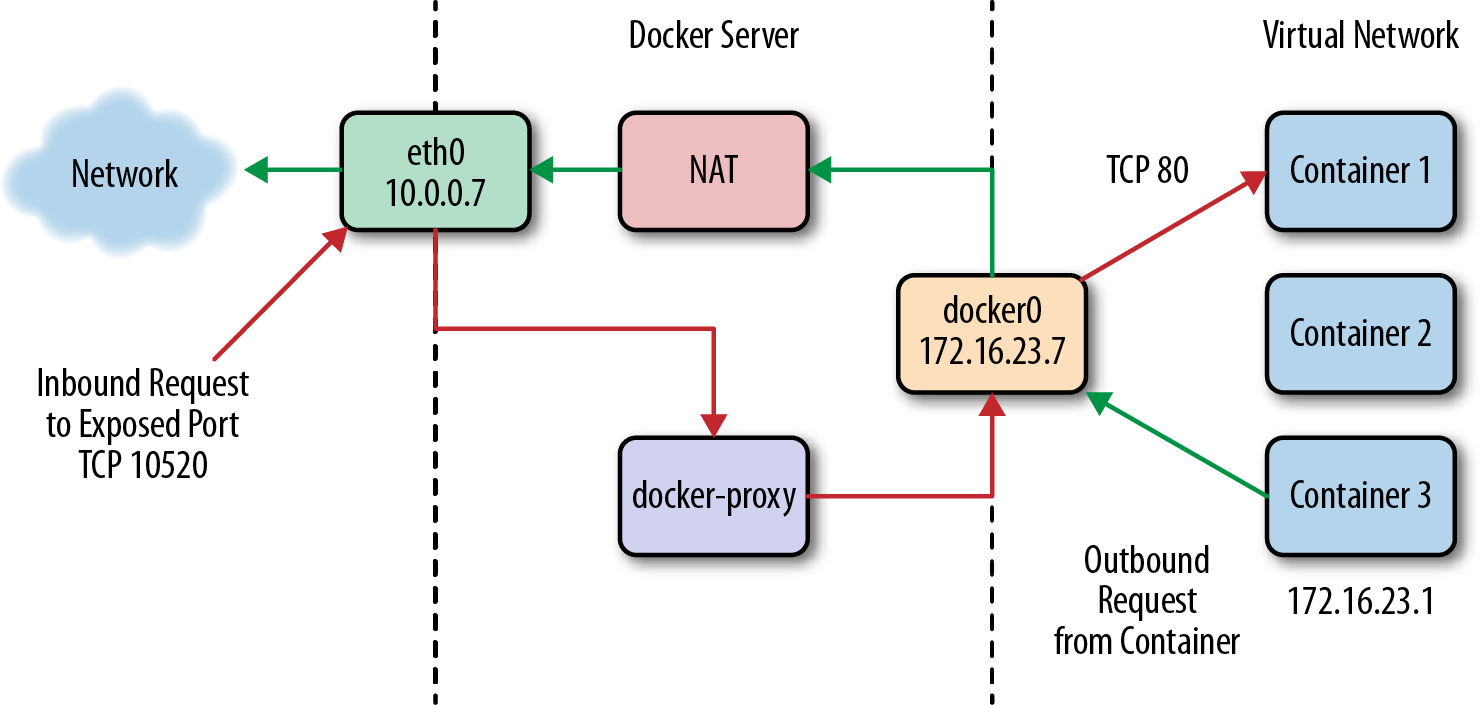
\includegraphics[width=.6\textwidth]{img/swarm-network}
\caption{Sieć dokera }  \label{rys:network}
\end{figure}

Na rysunku \ref{rys:network} \dots


\subsection{Dwa rysunki obok siebie}

\begin{figure}[ht] 
	\centering
	\begin{minipage}[b]{0.45\textwidth}
		\centering
\includegraphics[width=0.9\textwidth]{img/kotek} % left figure
		\caption{Lewy rysunek}\label{fig:lewy}
	\end{minipage}
	\begin{minipage}[b]{0.45\textwidth}
		\centering
		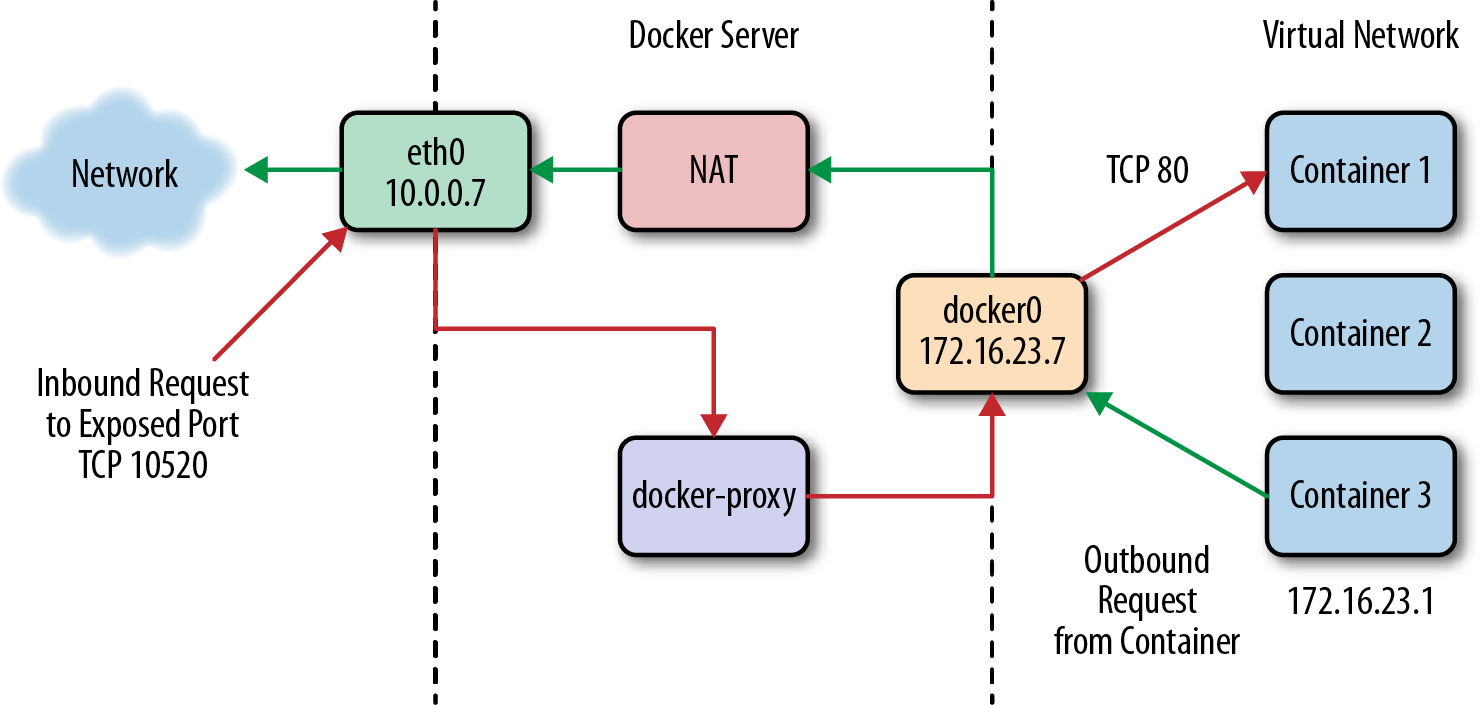
\includegraphics[width=0.9\textwidth]{img/swarm-network} % right figure
		\caption{Prawy rysunek}\label{fig:prawy}
	\end{minipage}
\end{figure}

Na rysunkach \ref{fig:lewy} i \ref{fig:prawy} \dots


\section{Tabele}

W tabeli \ref{table:table1} \dots

\begin{table}
\centering\caption{Tytuł tabeli (patrz dodatek~\ref{app1}) \label{table:table1}}
\begin{tabular}{|l|l|l|}% table alignment -> l c r - left, center, right
\hline
Pierwszy & Drugi & Trzeci \\
\hline
Pierwszy & Drugi & Trzeci \\
\hline
\end{tabular}
\end{table}

\subsection{Równania}

\begin{equation}
\sum_{i=1}^{\infty}a_i
\label{eq:myEquation}
\end{equation}

W równaniu \ref{eq:myEquation} \dots

\section{Listingi}

Na listingu \ref{listing:myListing} \dots

% replace {c} with the appropriate language
\begin{listing}
\begin{minted}{c}  
int main()
{
   int a=2*3;
   printf("**Ala ma kota\n**");
   while(!I2C_CheckEvent(I2C1, I2C_EVENT_MASTER_MODE_SELECT)); /* EV5 */
   return 0;
}
\end{minted}
\caption{Język C} \label{listing:myListing}
\end{listing}

